\graphicspath{{chapters/laboratory/07/images/}}
\chapter{Somatic copy number calling}

\section{Introduction}

	\subsection{Copy number mutations}
	Copy number mutations involve large portions of the genome.
	The spectra of deletions i much simpler to characterize: homozygous deletions are clear to spot, as no coverage is observed.
	For higher copy number the pattern is more difficult to identify as the combinatorial distribution in allelic distribution makes it difficult to recognize.

	\subsection{Effect of CNVs}
	CNVs are present in the population with different frequencies.
	Similarly as SNPs, CNVs can be associated with disease or with a specific phenotype.
	Their inheritance procedure is more complex with respect to the one of SNPs.

	\section{Circular binary segmentation}

		\subsection{Introduction}
		Circular binary segmentation CBS is an algorithm that analyse copy number data in array data.
		CNVs are detected by looking for change-points in array data, which are locations in data where the distribution changes.

		\subsection{Input}
		As input $N$ markers, representing the $\log_2 R$ of the intensities are given.
		The $\log_2 R$ corresponds to the signal for DNA in the tumour sample over the DNA signal in the control sample.
		Each point is the intensity of the signal of a probe in a microarray.
		Probes are ordered by gnomic coordinate.

		\subsection{An example}
		Considering $4$ examples of $\log_2 R$ data, it can be plotted as in figure \ref{fig:cbs}.

		\begin{figure}[H]
			\centering
			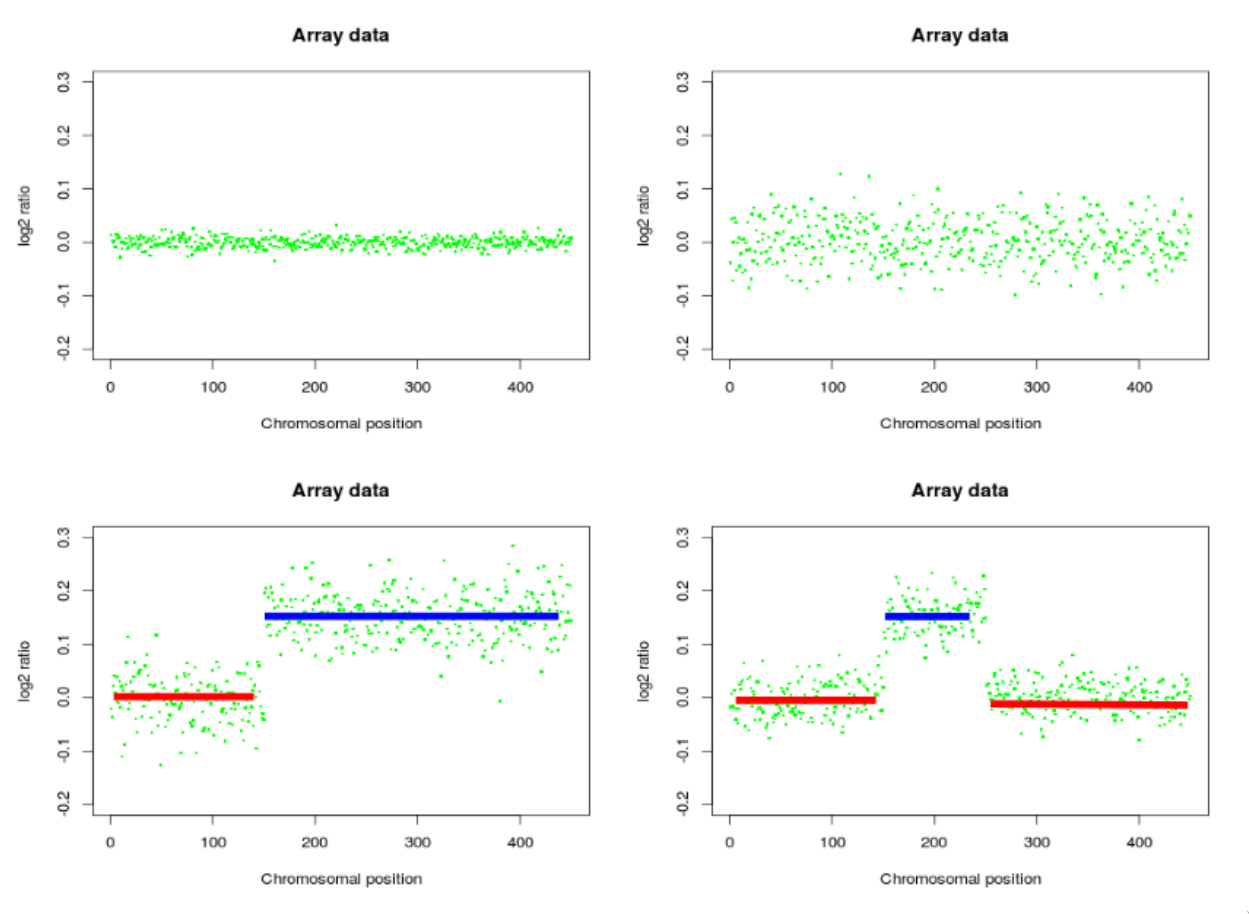
\includegraphics[width=\linewidth]{cbs}
			\caption{Four example of $\log_2 R$ distribution}
			\label{fig:cbs}
		\end{figure}

		The signal for the first line data shows no CNV, while in the second some noise can be seen.
		In the third the copy number variation involves the region from $150$ to $450$, while in the fourth the CNV only encompasses a smaller region.

		\subsection{Null hypothesis}
		The null hypothesis of CBS states that the arc from marker $i$ to marker $j$ and its complement have the same mean: absence of a CNV.
		It is rejected if the $p$-$value$ of the likelihood that the two arcs have the same mean is less than a parameter $\alpha$.

		\subsection{DNAcopy}
		DNAcopy is an R package for analysing array copy number data.
		DNAcopy splits a chromosome into regions of equal copy number.
		Calling copy number in somatic and germline is different since the method is based on the $\log_2 R$, a model representing a reference for germline variants is needed.
		This should be extremely well tuned to avoid false calls.
		Some bias can be present as the average value is not always the best one.
		Some databases for this approach are available, but there is no golden standard.

		\subsection{Changing parameters}
		Changing $\alpha$ could return a different result.
		Moreover in order to improve the quality in the case of over-segmentation, the option undo can be used to eliminate or collapse segments when there are not at least a number of standard deviations between segment means.
		Moreover outliers can be detected by smooth and deleted from the data.

		\subsection{Visualizing CNVs}

			\subsubsection{IGV}
			By writing data as a table, it is possible to export it to IGV as a seg file.
			The mean $\log_2 R$ value for each sample projected on the reference genome coordinate is visible.
			If blue it represents deletion, while if red amplification.
			A consensus for a specific region can be built.

			\subsubsection{Histogram}
			In order to better visualize the distribution of $\log_2 R$ segments in the sample an histogram can be built.
			A peak in $0$ is expected as the majority of the samples have the same copy number.
			The more signal, the more secondary peaks are expected for deletions and amplification.

			\subsubsection{Browsing a CNV across many individual}
			For browsing a CNV across many individuals the getSegments function can be used.
			A shift according to the reference is expected for germline variants.
			In the case of a rare CNV, a clearly higher zero peak is expected, while different peaks with similar height indicate a pretty common CNV.

\section{CNV calling in WES}
In whole exome sequencing only coding regions are captured.
The shape of the coverage is different across genes because the capture efficiency depends on technical parameters like high $GC$ content that results in lower coverage.
It is necessary to apply some corrections prior to variant calling.

	\subsection{Applying CBS}
	In order to apply CBS data needs to be cleaned and the $\log_2 R$ needs to be computed.
	This can be done on the coverage of the sample and the reference coverage once they have been normalized.
	Some tools include all the necessary framework, while others only modules.
	For example VarScan can take as input mpileup | copynumber and then applies copyCaller.
